\subsection{WP3 APAs (8 pages)}

{\bf Work package managers: J.\,Evans, A.\,Grant.}

\subsubsection{Introduction}

The APAs --- Anode Plane Assemblies --- are the most critical components of the TPC, collecting the ionisation charge for readout, allowing reconstruction of detector activity with mm-level resolution. These \SI{6x 2.3}{\metre} planes, one of which (built in the UK) is shown in Figure~\ref{fig:CompleteAPA}, have four layers of \SI{150}{\micro\metre} beryllium-copper wire wound around them, as shown in Figure~\ref{fig:APADiagram}. The layer structure is shown in Fig.~\ref{fig:APALayers}: from inside out, the layers are labeled $x$, $v$, $u$ and $g$. The $x$-layer and $g$-layer wires are aligned along the longest direction of the APA. The $v$-layer and $u$-layer wires are wound at an angle of \ang{35.7} to the the $x$-layer and $g$-layer. In between the inner $x$-layers, a grounding mesh is attached directly to the APA frame to prevent charge from within the APA from reaching the collection wires and producing `shadow' tracks. A full description of the construction and functionality of the APAs can be found in Chapter 2 of Volume 2 of the DUNE Interim Design Report~\cite{ref:DUNEIDR}. Once installed in the DUNE Far Detectors, the APAs will be hung vertically, in pairs hung one above another, as shown in Figure~\ref{fig:APAsInTheDetector}. The wires are read out by cold electronics at the top end of the top APA, and the bottom end of the bottom APA.

\begin{figure}
    \centering
    \includegraphics[width=0.6\textwidth]{figs/WP3/UKAPA.png}
    \caption{A complete protoDUNE APA, at the Daresbury Laboratory.}
    \label{fig:CompleteAPA}
\end{figure}

\begin{figure}
    \centering
    \includegraphics[width=0.6\textwidth]{figs/WP3/WireWindingAngles.png}
    \caption{The winding angles of the four wire layers.}
    \label{fig:APADiagram}
\end{figure}

\begin{figure}
    \centering
    \includegraphics[width=0.6\textwidth]{figs/WP3/WireLayers.png}
    \caption{The APA layer structure.}
    \label{fig:APALayers}
\end{figure}

\begin{figure}
    \centering
    \includegraphics[width=0.6\textwidth]{figs/WP3/TPCDiagram.png}
    \includegraphics[width=0.35\textwidth]{figs/WP3/HangingAPAs.png}
    \caption{Left: The layout of the TPC inside a \SI{10}{\kilo\tonne} FD module. Right: Two APAs hung, one above another, as they will be in the FD.}
    \label{fig:APAsInTheDetector}
\end{figure}

We propose to build 150 APAs in a factory at the Daresbury laboratory. This will be half of the APAs required for the first two \SI{10}{\kilo\tonne} single-phase Far-Detector modules. The UK factory will be the biggest in the DUNE Collaboration; the remaining 150 APAs will be produced at two or three (to be defined) other factories in the US. By delivering this very significant part of the TPC instrumentation, the UK have built its reputation as the most significant international partner in the Collaboration; we will also build up invaluable detector expertise that will allow UK physicists to be future Collaboration leaders.

The UK group that is proposing this project has demonstrated its ability to deliver by building two APAs for the protoDUNE detector. The protoDUNE APA construction was led by Evans and Grant, who will be leading this DUNE FD APA-production work package. The key technical staff working in this WP were closely involved in the protoDUNE construction. The UK technical staff have also been leading the development of the APA-production procedures, based on protoDUNE experience, to allow mass production for DUNE. In particular, Muir and Grant have redesigned the winding machine to speed up the wire-winding process. \todo{Mention SBND APAs?}


\subsubsection{Work plan}

This project follows on from the UK pre-production project. As part of this pre-production project, we have updated the APA-production procedure to allow mass production, and are building the first of the four new winding machines that will make up the Daresbury factory. We are also in the process of preparing the area in the Daresbury Electron Hall that will house the new factory.

WP3 begins at the start of the project, nominally on 1st October 2019. In the first nine months of the project, we will complete the build of the factory, assemble the remaining three winding machines and put in place all tooling and jigs. In this time, we will also define and document all quality-control procedures, and ensure full documentation of the APA-production procedures. We will also set up all procurement contracts.

APA production will begin on 1st July 2020. As detailed below, the factory will produce one APA every ten working days, which are shipped to SURF in pairs. The APAs for the first \SI{10}{\kilo\tonne} module will be complete on 1st August 2023. Those for the second \SI{10}{\kilo\tonne} module will be complete on 30th June 2026.

To mitigate the risk that the second \SI{10}{\kilo\tonne} module will not use the single-phase technology, all procurement contracts will be placed in two batches. Contracts for the first module will be placed at the start of the project; contracts for the second module will be placed as soon as the technology decision is made (expected in 2021\todo{Is this the right date?}). Procurement of APA frames is the biggest procurement task; it will be ongoing throughout the project with two frames intended to be delivered, on average, every 15 working days. \todo{Is this right, Alan?} The remaining large procurement tasks (mesh panels and electronic components) will be complete by 2023, and the fully-tested components stored until needed.

\subsubsection{WP3.0 Management}

Managers: J.\,Evans, A.\,Grant.\\
This sub-WP runs for the entirety of the project. It effectively ends with the installation of the final UK APA into the DUNE Far Detector.\todo{not quite, lessions learned,....}

\paragraph{WP3.0.1 Overall management} Managers: J.\,Evans, A.\,Grant.

Overall management for the work package will be provided by academic Evans (70\% FTE on the project) and project manager A.\,Grant (100\% FTE on the project). Evans and Grant oversaw the production of the UK protoDUNE APAs, and have been leading the UK pre-production project that has delivered the new winder design, new APA mass-production procedures, and setup of the Daresbury factory infrastructure. 

Evans will focus on overall management of the Work Package, ensuring the UK groups are working together efficiently, that the correct people are hired into posts and that staff changeover is handled proactively. Evans will also be responsible for representing the Work Package to the international collaboration, primarily through the DUNE APA Consortium (which is led by Touramanis).

\paragraph{WP3.0.2 Quality management} Manager: Quality Manager\todo{also describe what kind of person this is}.

Strict quality-assurance procedures must be put in place from day one of the project. A dedicated Quality Manager will be employed to manage this aspect of the project. They will be responsible specifying and documenting the quality-control procedures at the start of the project, for ensuring the procedures are followed during production, and for documenting all quality-control data. The Quality manager will work closely with the US groups that are building APAs, in particular the PSL group where many procedures have been defined, to ensure that uniform procedures and requirements are defined across all APA factories.

Hiring of the Quality Manager will be one of the first high-priority tasks in the project; the job description will require the person to have previous experience in quality management.
The Quality Manager will be implicitly involved in all the sub-WPs described below, and will be expected to be mobile: actively working with all the UK groups to assure quality in their areas of responsibility. The Quality Manager will be employed full time for the first three years of the project as the procedures are defined and the discipline of following the procedures instilled in the team. After this, the Quality Manager will drop to a 50\% FTE position, which will be adequate to allow continued oversight.

\paragraph{WP3.0.3 Procurement management}

Manager: A.\,Grant

The major procurement activities will make use of the professional procurement teams in place at the Universities: APA frames (Liverpool), Electrical components (Manchester), mesh panels (Sheffield). All other equipment will be procured by the Daresbury Laboratory. High-level oversight for all procurement activities will be provided by A.\,Grant, and overall project manager Preece. In the first year of the project, Gamez (deputy factory manager, and experienced member of the protoDUNE APA-production team) will focus a significant amount of time on supporting the procurement activities.\todo{we will need more substance on procurement, not sure if it is here or in the management section.}

Procurement is explicitly written into the work-package breakdown described below, with engineering and physicist staff assigned responsibility for the major procurement tasks. In the first nine months of the project, the main focus of these staff will be on the tendering process, visiting potential suppliers to ensure they can achieve our requirements. Once production is underway, the staff responsible for each procurement contract will work closely with the suppliers, visiting on a weekly basis if necessary, to ensure QC procedures are followed and requirements are met.

As mentioned earlier, to mitigate our exposure to the risk arising from the outstanding technology decision for the second \SI{10}{\kilo\tonne} module, the first set of procurement contracts will be placed for the equipment for 75 APAs. The contracts for the second 75 APAs will be placed once the technology decision has been made.\todo{repetition, may be dropped}

\paragraph{WP3.0.4 Communication with the international collaboration}

Manager: J.\,Evans.

As part of the overall management, Evans will represent the WP to the UK collaboration and the international DUNE collaboration. Within the UK project, Evans and A.\,Grant are part of the Project Management Committee, through which formal communication with the international collaboration will occur. They report directly to the project PI. 

Evans will coordinate WP activities with the international collaboration through the APA Consortium (led by Touramanis), ensuring regular reporting of UK activities. The APA consortium will also provide the mechanisms by which the UK team is informed about APA-production activities in the US. A close working relationship has already been built up between the UK and US teams that will continue into the construction phase.

A particular focus of this WBS element will be the tracking and implementation of technical decisions taken by the wider collaboration, whether this be a small update to the APA design, or a major decision such as an FD module technology choice.

\subsubsection{WP3.1 APA mechanics}
Managers: T.\,Jones, P.\,Sutcliffe.\\
This sub-WP runs for the duration of the grant. It ends when all mechanical parts of all APAs are at Daresbury, fully tested and ready for installation onto an APA.

\paragraph{WP3.1.1 APA frames} Manager: P.\,Sutcliffe.

The APA frame is a \SI{6x2.3}{\metre} stainless steel structure, as shown in Figure~\ref{fig:APAFrame}. The individual bars are selected from commercial section, end fittings welded on, and the whole frame screwed together on a jig that ensures flatness to the requirements listed in Tab.~\ref{tab:APAFlatness}.

\begin{figure}
    \centering
    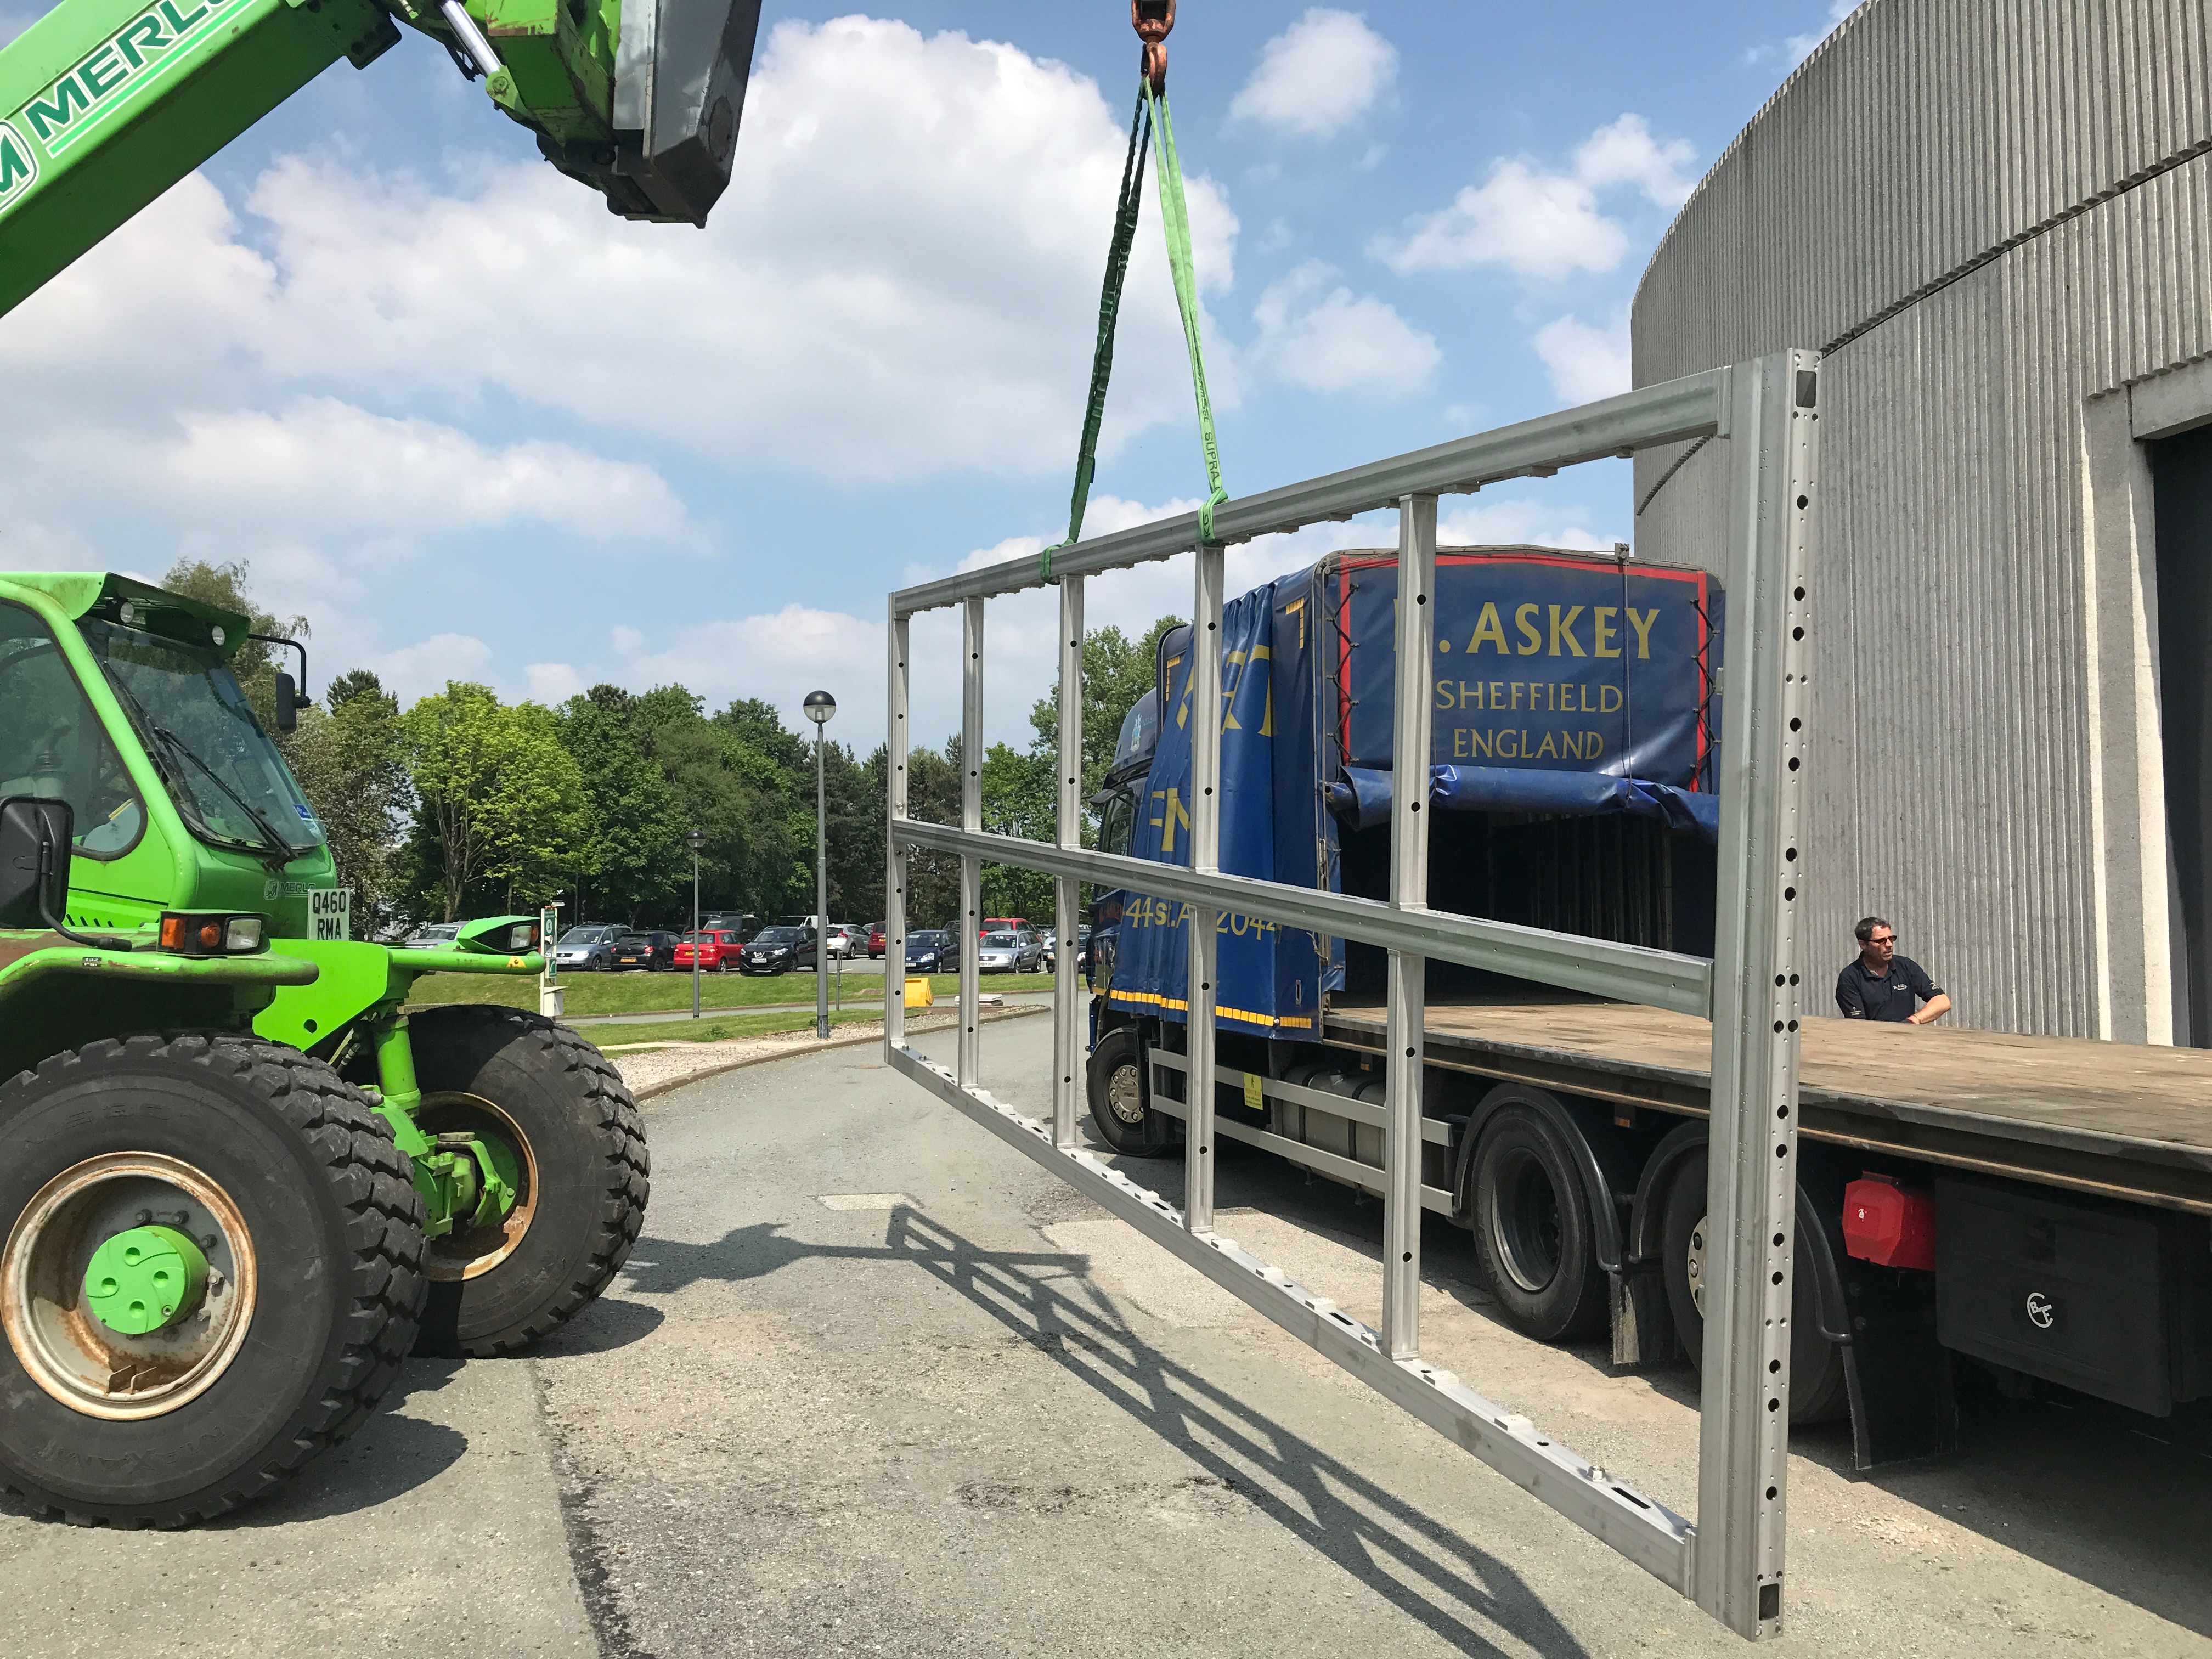
\includegraphics[width=0.6\textwidth]{figs/WP3/APAFrame.png}
    \caption{A protoDUNE APA frame.}
    \label{fig:APAFrame}
\end{figure}

\begin{table}
\centering
\begin{tabular}{|l|c|}
\hline
    \multicolumn{1}{|c|}{\bf Criterion} & {\bf Tolerance} \\ \hline
    \multicolumn{2}{|c|}{\bf Flatness}\\
    Overall flatness & \SI{11}{\milli\metre} \\
    Overall bow & \SI{11}{\milli\metre}\\
    Overall twist & \SI{2}{\milli\metre / \metre}\\
    Twist in each zone of the frame & \SI{2}{\milli\metre / \metre}\\ \hline
    \multicolumn{2}{|c|}{\bf Fold --- front and back sides}\\
    Foot tube & \SI{1.2}{\milli\metre}\\
    Head tube & \SI{1.2}{\milli\metre}\\
    Ribs 1--4 & \SI{1.2}{\milli\metre}\\
    \hline
\end{tabular}
\caption{APA flatness requirements}
\label{tab:APAFlatness}
\end{table}

The DUNE frame design will be very similar to the protoDUNE design. The only change being made is that the width of the steel section is being increased to allow cables to be run along the insides of the frame sections. This change will require some alternations to the deigns of the geometry boards (the PCBs onto which the wires are attached), but will not require any changes to the APA production procedure. The international collaboration intends to finalise the APA frame design by the end of 2018\todo{Is this true}, so this will not delay the start of the UK project.

The engineers responsible for delivering the APA frames will be Peter Sutcliffe (supported by Liverpool\_Eng), a highly experienced mechanical engineer who currently leads the DUNE APA Consortium's testing, installation and integration working group, and Trevor Gamble, the mechanical engineer who oversaw the production of the UK APA frames for protoDUNE. Additional oversight will be provided by T. Jones, who is highly experienced in managing large experimental construction projects such as the ATLAS Upgrade, and Payne who delivered the SBND CPA, supported by Liverpool\_AP. PDRA effort at Liverpool and Sheffield is assigned to this task to perform analysis of QC data (such as laser survey data); technician effort is also assigned at Liverpool and Sheffield to support the work.

To ensure that the frame supply is reliable, we will place contracts with two or three suppliers who will make frames in parallel. We expect to receive, on average, four frames every 30 working days.
In the first nine months of the project, close to 3.5 FTE is assigned to the setting up of the procurement contracts: visiting potential suppliers, defining QC procedures, and working with chosen suppliers to set up the procedures. Once the APA production is in full flow, this drops to around 3 FTE: every month, a team will spend five days on the premises of each of the suppliers, working with the supplier to perform QC on the frames. By working with the supplier like this, we maintain control of this most criticial piece of QC; as a byproduct we also save money as the suppliers will not have to charge as much for the QC of the frames. To perform the frame QC, we will purchase a laser survey system such as a FARO Vantage, as part of the pre-production project. We budget £25k (plus VAT and contingency) to replace this system mid-way through the project to mitigate against its failure. This WBS element also includes oversight of shipping of completed frames to Daresbury, and dealing with any non-conformancies found in the frames at Daresbury.

\paragraph{WP3.1.2 Mesh panels} Manager: T.\,Gamble.

A significant improvement on the protoDUNE APA production procedure is the use of UK-designed mesh panels, shown in Fig.~\ref{fig:MeshPanel}, that quickly and easily slot into the APA frames, reducing the production time of an APA by three days. We are currently fitting these mesh panels to the seventh protoDUNE APA (which will be used as an electronics test-stand) to ensure there are no unforeseen installation or operational issues.

\begin{figure}
    \centering
    \includegraphics[width=0.4\textwidth]{figs/WP3/MeshPanel.png}
    \caption{A mesh panel.}
    \label{fig:MeshPanel}
\end{figure}

The same technical team as is producing APA frames will be responsible for the mesh panels, though with formal responsibility at Sheffield rather than Liverpool, to ensure dedicated oversight. The mesh panels will be procured and tested in the first four years of the grant, then stored until needed.
\todo{Would be nice to say something quantitative about requirements and tolerances.}

\paragraph{WP3.1.3 APA parts procurement} Manager: D.\,Gamez.

A wide array of smaller mechanical parts are needed to produce an APA. This includes the beryllium-copper wire, the combs and comb-bases that maintain the wire spacing, epoxy, solder, and the APA protection panels that surround the APA before it goes into the shipping box. Overall responsibility for ensuring the supply of all these components will fall with Gamez (supported by Manchester\_AP), who will be the deputy factory manager. Gamez was the lead PDRA for the protoDUNE APA production so is intimately acquainted with the required materials and therefore ideal to move into this core management position.

The first nine months of the project will see the search for suppliers who can provide materials at the rate required to keep the factory in stock. Once APA production is underway, WP3.4.3 details the responsibilities of the technical staff to monitor the level of materials at the factories. And shortages will be reported to Gamez, and the responsibility lies in this WBS element to maintain the supply.

\subsubsection{WP3.2 Electrical components}

Managers: J.\,Pater, M.\,Perry.\\
This sub-WP runs for the first four years of the project. It ends when all electrical components are fully tested and in storage, ready for installation onto an APA.

\paragraph{WP3.2.1 PCB and cable procurement}

Manager: J.\,Pater.

Explain how many different types of boards there are.
State the QC requirements.
All done in the first four years.

\paragraph{WP3.2.2 PCB and cable reception testing}

Manager: M.\,Perry.

Need to talk to PSL.

\paragraph{WP3.2.3 Board assembly}

Manager: M. Perry.

Need to talk to PSL.

\subsubsection{WP3.3 Factory setup}
Manager: A.\,Grant.\\
This sub-WP runs for the first nine months of the project. It ends when the factory setup is complete, and all four production lines have begun operations.

\paragraph{WP3.3.1 Factory infrastructure} Manager: A.\,Grant.

The APA factory, shown in Fig.~\ref{fig:APAFactory}, will be in the Electron Hall at the Daresbury Laboratory.\todo{Perhaps give the floor area?} Work is already underway to prepare the area, repairing the floor, installing new cranes, and all infrastructure needed such as power and the clean area. A.\,Grant will oversee this WBS element, aiming to have the factory area ready for installation of winding machines by October 2019.

\begin{figure}
    \centering
    \includegraphics{figs/WP3/FactoryLayout.png}
    \caption{The APA factory at Daresbury.}
    \label{fig:APAFactory}
\end{figure}

This WBS element also covers the purchasing of the access tooling needed for production (ladders, working platforms), the installation of storage racks, and the setting up of materials-preparation tables.


\paragraph{WP3.3.2 Winding machines} Manager: A.\,Muir.

The DUNE winding machine was originally designed by engineers at PSL (Madison, Wisconsin), and has been improved upon by UK engineers, led by Muir, to allow a much faster winding process with significantly less handling of the APA, and improved wire-tension control. The first of the new winding machines has been built at Daresbury (Fig.~\ref{fig:WindingMachine}), and is now being commissioned. This will be the first of the four winding machines in the Daresbury factory. Over the next three months\todo{give dates as it is not clear when the document will be read.}, it will be used to wire a seventh protoDUNE-style APA, which will be used as an electronics test stand. This winding exercise will allow us to run through all the new production processes, and to iron out any problems with the new winding machine.

\begin{figure}
    \centering
    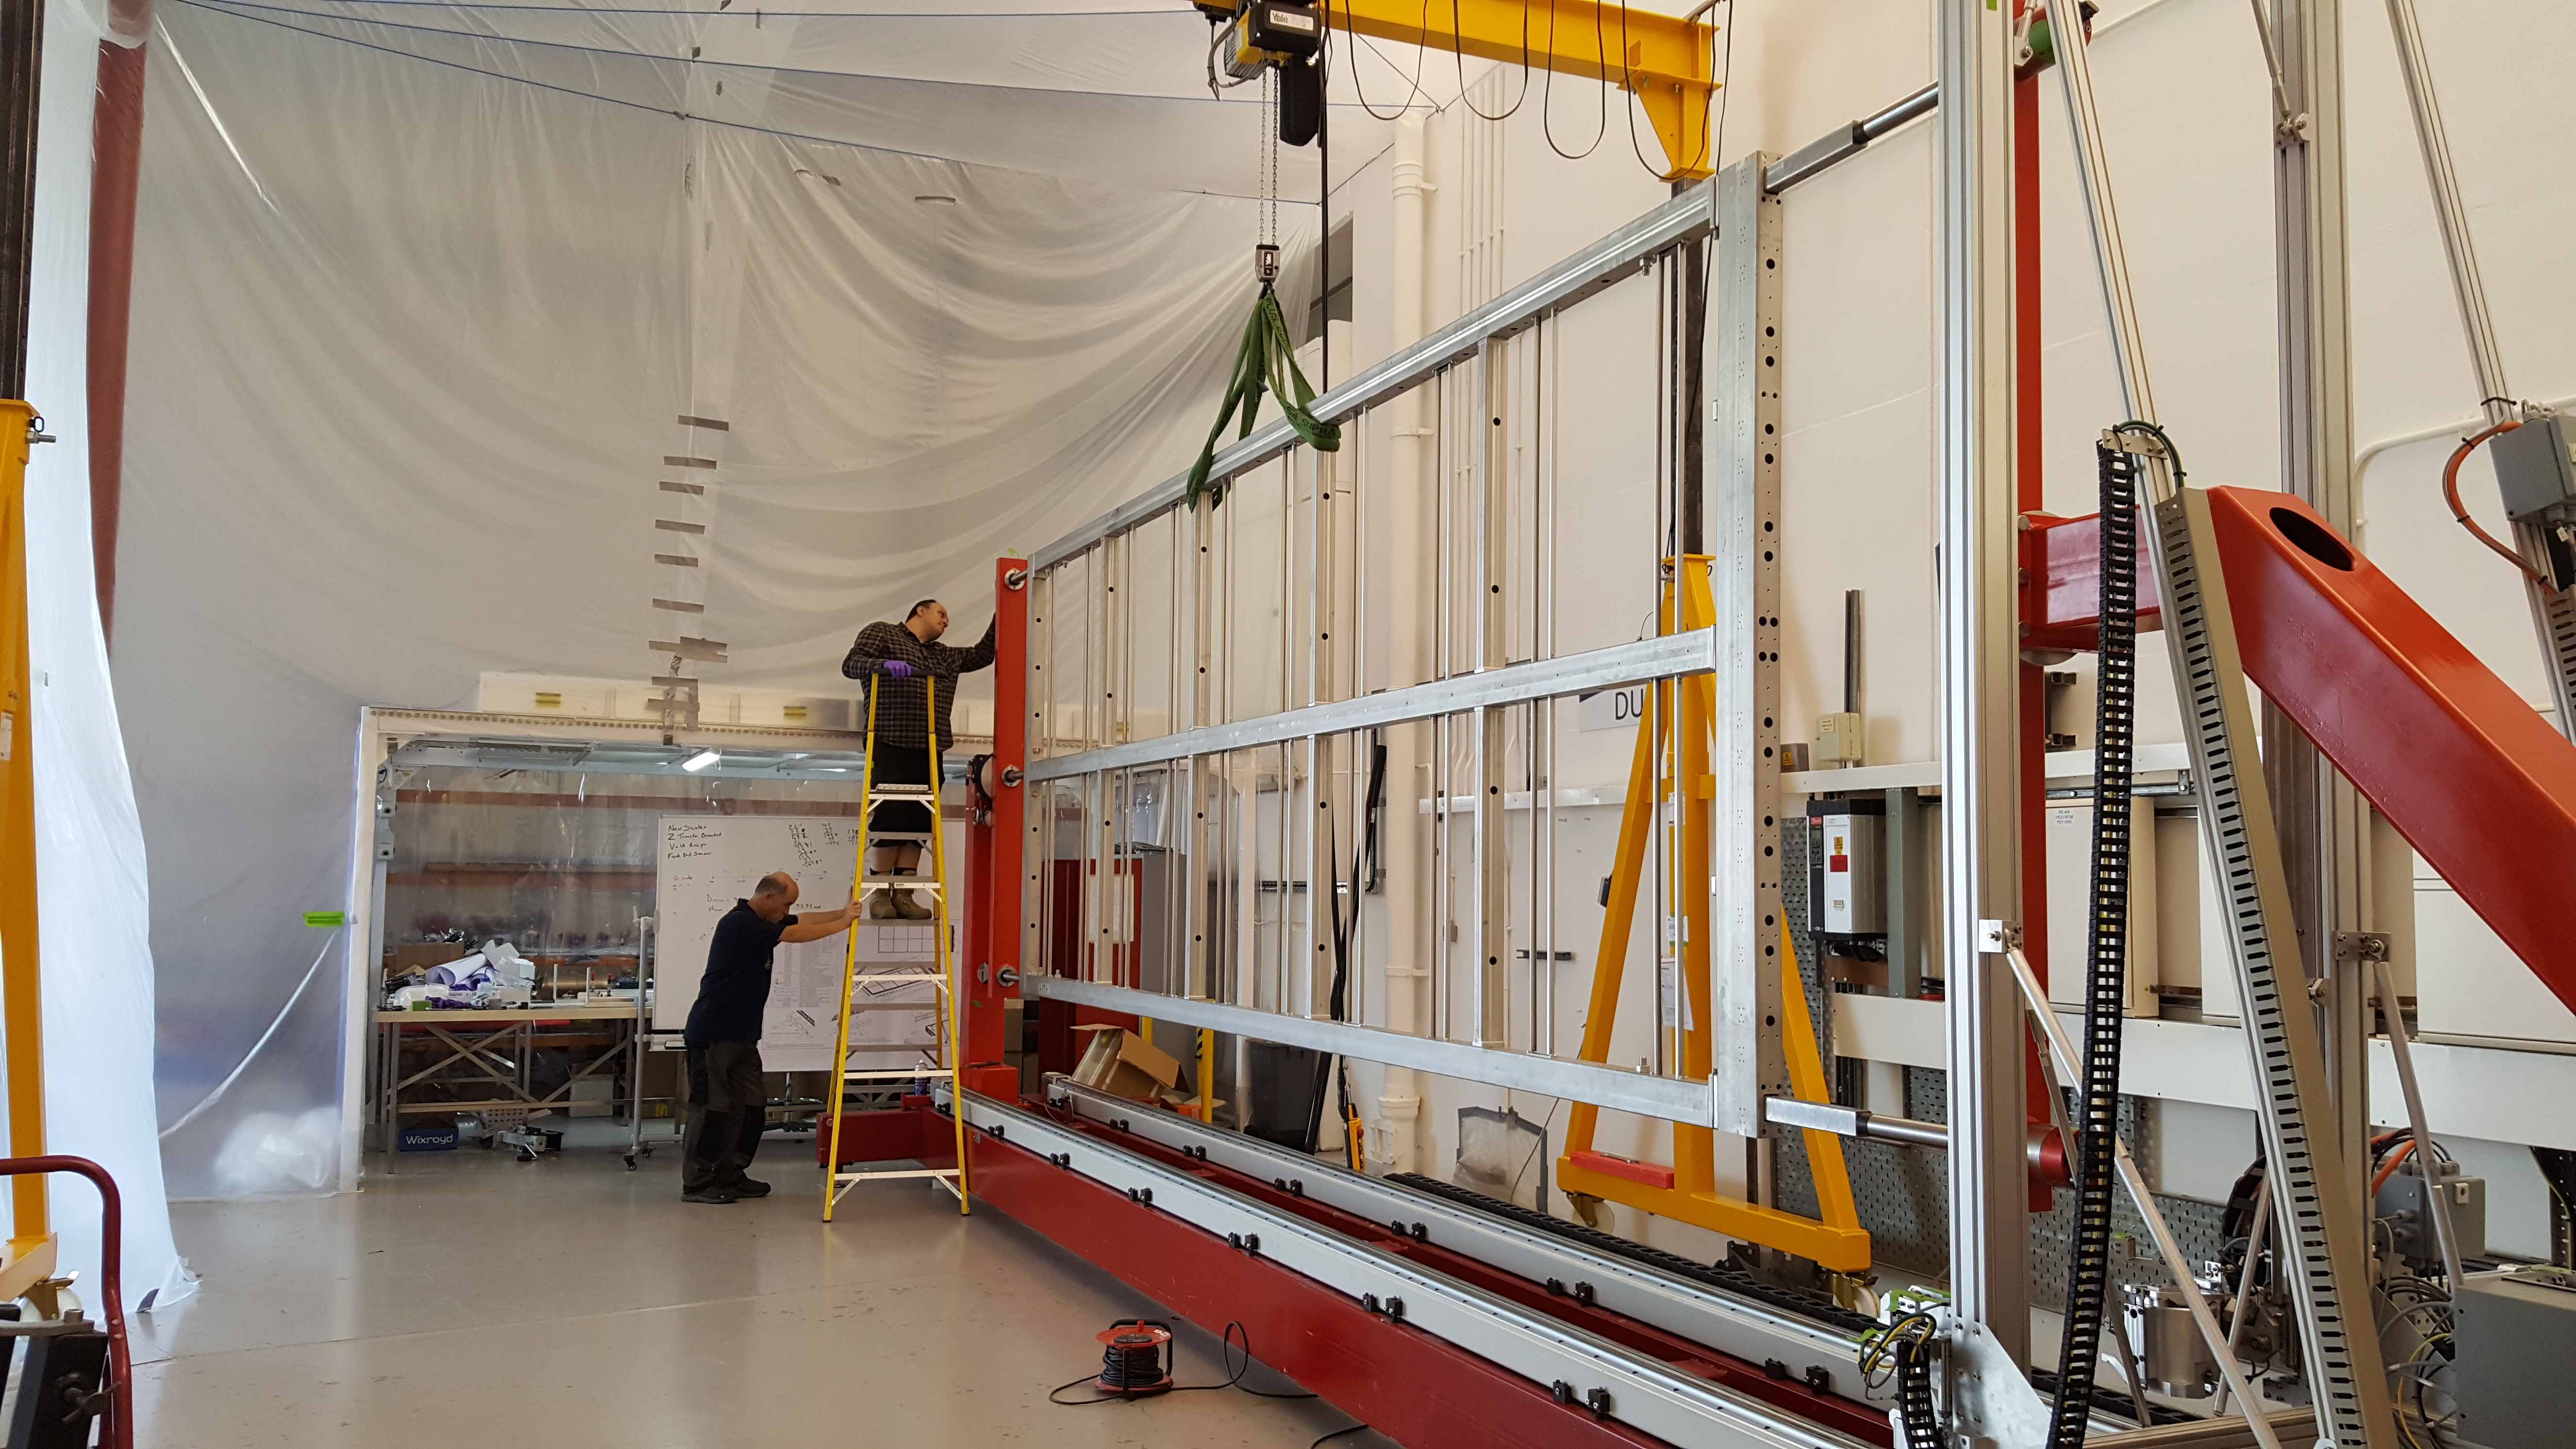
\includegraphics[height=0.3\textwidth]{figs/WP3/TheNewWinder.jpg}
    \includegraphics[height=0.3\textwidth]{figs/WP3/ActiveTensionHead.png}
    \caption{Left: the DUNE winding machine. Right: the winding head with active tension control.}
    \label{fig:WindingMachine}
\end{figure}

The Daresbury factory will consist of four winding machines. This WBS element will see Muir oversee the build of the three remaining machines in the first nine months of the project, and the move of the existing machine down from the Daresbury Tower area to the factory area.

\paragraph{WP3.3.3 Process carts and jigs} Manager: A.\,Muir.

Before and after winding, the APAs are handled on process carts (Fig.~\ref{fig:ProcessCart}). As well as allowing the APAs to be moved around the factory, these process carts are where photon-detector rails and mesh panels are installed, and where cover boards and APA protection panels are installed. We have two process carts, and will purchase a further 8. This will give us two process carts per winding machine, and two additional ones to allow complete APAs to be moved around the factory and taken to the shipping area.

\begin{figure}
    \centering
    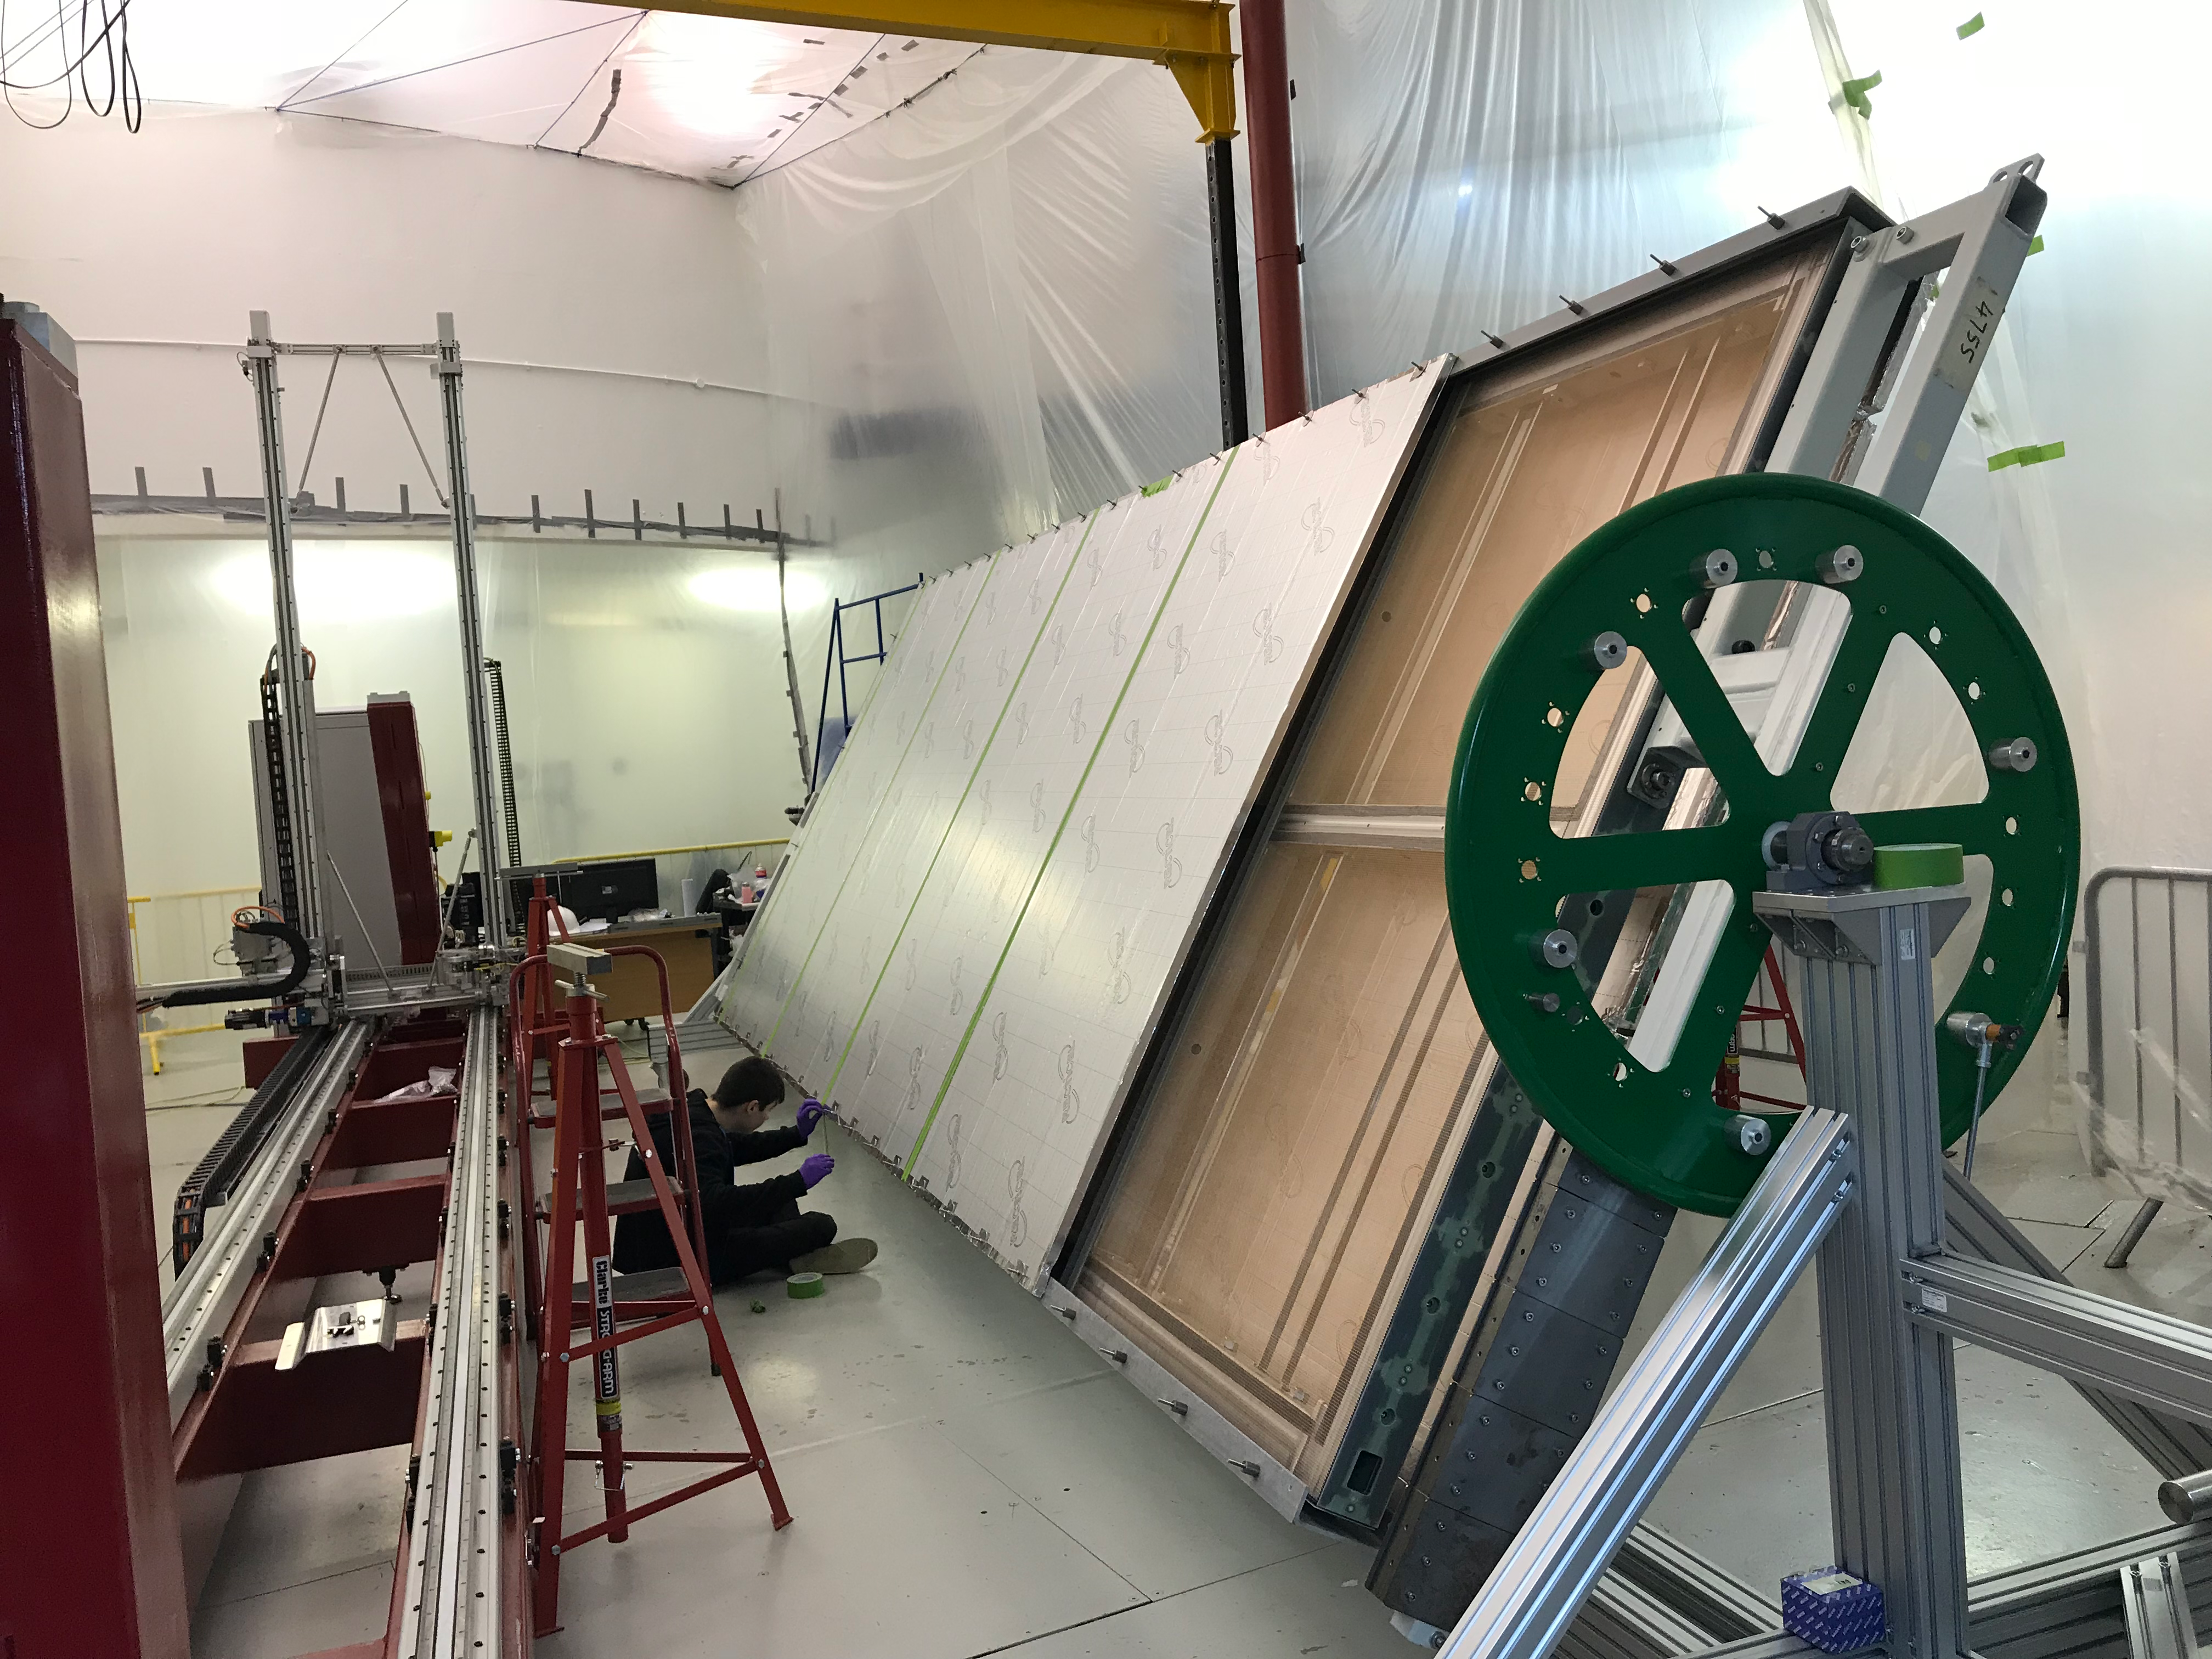
\includegraphics[width=0.6\textwidth]{figs/WP3/ProcessCart.png}
    \caption{An APA on a process cart, being prepared for shipping.}
    \label{fig:ProcessCart}
\end{figure}

This WBS element includes the purchase and construction of all the jigs required for APA construction, such as comb-assembly and comb-installation jigs, tooling for installing mesh panels, and jigs for applying epoxy to the geometry boards.

\subsubsection{WP3.4 Factory operations} Managers: D.\,Gamez, A.\,Grant.\\
This sub-WP begins in month 10 of the project, and runs to the project end. It begins when construction of the first APA starts in the factory; it ends when the final APA is shipped out of the factory.

\paragraph{WP3.4.1 Factory management} Managers: D.\,Gamez, A.\,Grant.

A.\,Grant will take the role of Factory Manager, and D.\,Gamez that of Deputy Factory Manager. Between them, they will provide full-time oversight of factory operations. They are both highly experienced in APA production from the UK protoDUNE activities.

\paragraph{WP3.4.2 Factory maintenance} Manager: A. Muir.

Maintaining the functionality of all four winding machines and their associated production lines, plus the factory infrastructure, is vital to maintaining the project schedule. Around 2 FTE is dedicated to factory maintenance throughout the project, a mixture of technician, engineer and PDRA effort. Technician effort will focus on the maintenance and replacement of the various jigs. At Daresbury, specialist electronics, mechanical and controls engineer time is dedicated to maintaining the winding machine. The first ports of call for winder software problems will be the specialist winding technicians, and Manchester\_PDRA who will be an expert in the winder controls software. Effort from university engineering staff is also ringfenced to be called on for factory maintenance: in case of a serious problem with a winder, an all-hands-on-deck attitude will be taken to get the factory running again as quickly as possible.

\paragraph{WP3.4.3 Materials management} Manager: D.\,Gamez.

It is vital that the factory not be starved of materials. Gamez (the deputy factory manager) will be responsible for overseeing the management of all materials supply. 50\% of one of the factory technicians will be dedicated to stock-keeping. When orders of new materials are required, this WBS element will feed into the relevant parts of WP3.1 and WP3.2 where procurement and supply of parts will be performed. 

\paragraph{WP3.4.4 APA production} Manager: A.\,Grant.

APA production is the central WBS element of the project. The factory consists of four production lines. Each production line is one winding machine and two process carts. The schedule for building a single APA is shown in Fig.~\ref{fig:FactorySchedule}, in terms of eight-hour shifts. It is assumed that the factory will run a single eight-hour shift with all four production lines in use on all standard working days. This then allows weekends and double-shifting to be used to regain any lost schedule.\todo{We need a bit more information so that the reviewers get a fuzzy feeling that we are on top of these estimates. Say how this was determined, which saving have been assumed and how much time/effort contingency has been added.}

\begin{figure}
    \centering
    \includegraphics[width=\textwidth]{figs/WP3/FactorySchedule.png}
    \caption{The schedule for producing a single APA.}\todo{this has to be readable, needs higher resolution}
    \label{fig:FactorySchedule}
\end{figure}

The schedule driver is the 40 shifts (i.e. 40 days in the default schedule) that the APA spends on the winder. We therefore aim to keep the winders in use at all time. Prior to winding, pre-production activites take place on a process cart; post-production on a second production cart. By having two production carts paired with each winding machine, whilst the $n$th APA is on the winding machine, pre-production on the $(n+1)$th APA and post-production on the $(n-1)$th APA can take place. Thus the factory can produce four APAs every 40 working days.

The core technician team consists of 13.5 technicians who will be based full-time at the Daresbury factory. Seven of the technicians, along with the 50\% technician, are assigned 100\% to APA production, and will be the expert winder operators. The other six full-time technicians are assigned 50\% to APA production, focusing on the pre-winding and post-winding activities on the process carts. The other 50\% of the time of these six technicians are assigned to QC documentation, factory maintenance, materials management and shipping.

%Daresbury: 3.5, 1.5 is just winding. 2x0.5 is production, with maintenance and materials.
%Lancaster: 2 techs, both 50\% QC
%Liverpool: 2 techs, both 100\% production
%Manchester 3 techs: 1 is 100\% production, the other two shipping and maintenance
%Sheffield: 3 techs, 100\% production

In addition to the core technician team, fractions of university technical staff and PDRAs are earmarked for APA production so that we can call on them to cover holidays and sickness of members of the core team. We will also make use of PhD students as necessary to maintain the schedule.


\paragraph{WP3.4.5 APA quality control and documentation} Manager: Quality Manager.

The QC procedures will have been defined in WP3.0.2. This WBS element is where the APA production team follow the QC procedures, take any remedial action, document the results and produce non-conformance documents as required. The documentation will take the form of travellers that stay with the APAs. For protoDUNE, paper travellers were used. For DUNE, the Quality Manager will oversee the development of online iPad-based traveller forms that will allow easier storage of QC data in databases, and which can be rolled out to the US factories.

\subsubsection{WP3.5 APA shipping} Managers: D.\,Gamez, T.\,Jones.\\
This sub-WP runs through the entirety of the projet, ending when the last UK APA has been delivered to SURF and signed off as ready for installation.

\paragraph{WP3.5.1 Shipping boxes} Manager: J.\,Freestone.

An APA transport frame is shown in Fig.~\ref{fig:TransportFrame}. This holds two complete APAs and fits inside a standard shipping container. Engineers from Manchester and Liverpool will work together at the start of the project to find suppliers that can provide the transport frames at the required rate. Technical effort has also been assigned at the universities for final assembly of the transport frames.

\begin{figure}
    \centering
    \includegraphics[width=0.6\textwidth]{figs/WP3/APATransportFrame.png}
    \caption{A transport frame that holds two completed APAs.}
    \label{fig:TransportFrame}
\end{figure}

\paragraph{WP3.5.2 Shipping management} Manager: D.\,Gamez

Transport of completed APAs will be by ship across the Atlantic, then by road to SURF. Transport can begin as soon as the Integration and Test Facility (ITF) is available at SURF, currently scheduled for April 2021. Before this time, completed APAs will be stored in commercial storage in the UK. Once shipping begins, APAs will be shipped out of the factory as soon as a pair of APAs is ready to fill a shipping container.

The APAs will instrumented with vibration monitors. PDRA effort is assigned to analyse the data from these monitors. Any findings from these, or findings of damage at the ITF, will be fed back to the engineers responsible for the shipping boxes (WP3.5.2) who will make any necessary changes to the design.

\subsubsection{WP3.6 Integration}
Managers: N.\,McConkey, P.\,Sutcliffe.\\
This sub-WP runs for the full period of the project, and ends when the final UK APA is installed into the DUNE Far Detector.

\paragraph{WP3.6.1 Contributions to technical coordination} Manager: A. Muir.

Engineer effort dedicated to working as part of the international collaboration's technical coordination team can be reclaimed against the Common Fund requirement as a contribution in kind. 80\% of Muir, once the factory has been set up, is assigned to working for the collaboration's technical coordinator.

\paragraph{WP3.6.2 Detector studies} Manager: N.\,McConkey.

As production progresses, questions will arise about the APA design. There will also be non-conformances in APAs, and studies will be needed to understand whether the non-conformance can be accepted, or whether it will have to be recitified. PDRA effort is assigned to performing these studes.

\paragraph{WP3.6.3 APA reception testing at SURF} Manager: N.\,McConkey.

It is vital that UK physicists, in particular PDRAs, have a presence at SURF during construction, both to engage the UK in the installation and to build the reputation of our PDRAs within the international collaboration. Each PDRA requested in this WP will spend one year on LTA at SURF working with the integration teams there, focusing on APA reception testing.

\subsubsection{Deliverables and Milestones}

Alan and Roy: can you write this?

\subsubsection{Business Case}

This WP will engage a significant amount of UK business, in particular the production APA frames, PCBs, mesh panels and shipping boxes. We will be working in those companies, building their capability in the data-analysis involved in quality assurance.\todo{this needs to be extended. Use information from Benefit Realisation WS.}